\documentclass{article}
\usepackage[T1]{fontenc}

\usepackage{graphicx}
\usepackage{listings}
\begin{document}

\title{FOSS Lab Report}
\author{Gokul K\\[2\baselineskip]
Roll Number: 21\\[2\baselineskip]}
\date{02 February 2020}

\maketitle

\setcounter{section}{16}
\section{Shell Programming XIII}
\subsection{Aim}
Write a shell script that folds long lines into 40 columns. Thus any line
that exceeds 40 characters must be broken after 40th ; a\ is to be
appended as the indication of folding and the processing is to be
continued with the residue. The input is to be through a text file created
by the user.


\subsection{Source Code}
\begin{verbatim}
    #! /bin/bash

    # Gokul K
    # Roll No: 21
    # 25-01-2020

    # Write a shell script that folds long lines into 40 columns. Thus any line
    # that exceeds 40 characters must be broken after 40th ; a\ is to be
    # appended as the indication of folding and the processing is to be
    # continued with the residue. The input is to be through a text file created
    # by the user.

    if [[ $# -ne 2 || !(-f $1) ]]
    then
        echo "Please provide valid input filename and desired output filename"
        exit
    fi

    cat $1 |
    while read line
    do
        i=0
        echo $line |
        while read -r -n1 char
        do
            i="`expr $i + 1`"
            if [[ i -eq 40 ]]
            then
                printf "\n%s" $char >> $2
                i=1
            elif [[ $char = "" ]]
            then
                printf " " >> $2
            else
                printf "%s" $char >> $2
            fi
        done
    done

\end{verbatim}

\subsection{Program Description}
Each line in the file is looped through. Individual characters are parsed from them
and a counter counting up to 40 is established. After 40 a line break character is 
outputted before the 40th character, hence folding the line to 40 character.

\subsection{Output}
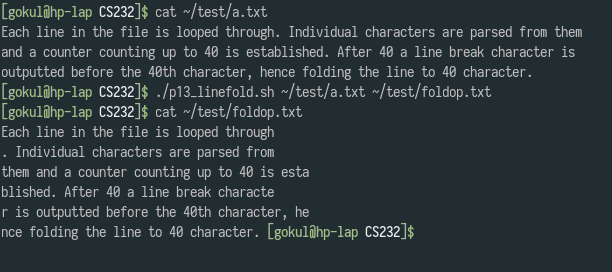
\includegraphics[width=0.9\textwidth]{img/p17.png}\newline

\subsection{Result}
The above program is run on Manjaro Linux shell. Lines in the input file was
folded to the 40 character limit and output was redirected to a file given as 
argument.
\end{document}